En este capítulo se presentan los diferentes requerimientos iniciales definidos por el cliente y por \textbf{Code Eaters}. En la primera sección se encuentran las necesidades del cliente expuestas en tablas describiendo su urgencia así como su dependencia de los requerimientos del sistema. En la segunda sección se encuentras aquellos requerimientos, siguiendo la clasificación de Frank Tsui de requerimientos funcionales, con los que el sistema contará al finalizar la primera iteración, expuestos en forma de tabla. En la tercera sección se encuentran expuestos los casos de uso. Cada conjunto de requerimientos está dividido de acuerdo a las necesidades cada uno de los stakeholders expuestos en el capítulo \ref{ch:Contexto}.

\section{Requerimientos iniciales del Usuario}

	\subsection{Dueño}
	
		\begin{ReqUser}
			\reqUserItem{RU-MI01}{Gestionar Tiendas}{El dueño de la empresa requiere de un mecanismo que le permita ver las ventas realizadas por las tiendas así como dar de alta nuevas o editar su domicilio geográfico, la capacidad de su almacén.}{\alta}{}
		
			\reqUserItem{RU-MI02}{Solicitar Inventario}{El dueño de la empresa requiere de un mecanismo que le permita comunicarse con el encargado de cada una de sus tiendas para que se lleve a cabo la actualización del inventario de cada almacén.}{\alta}{}
		
			\reqUserItem{RU-MI03}{Administrar Solicitudes de Producto}{El dueño de la empresa requiere de un mecanismo que le permita visualizar todas las solicitudes de producto hechas por cada una de sus tiendas y realizar la compra de cada una de ellas buscando el proveedor que más se adecue a sus necesidades en el momento de consulta.}{\alta}{}
		
			\reqUserItem{RU-MI04}{Consultar Entregas}{El dueño de la empresa requiere de un mecanismo que le permita conocer el momento en que se llego una entrega de productos a una tienda, fecha , hora y persona que recibió para comprobar que los productos que ingresaron hayan estado en las mejores condiciones.}{\alta}{}
		
			\reqUserItem{RU-MI05}{Gestionar Proveedores}{El dueño de la empresa requiere de un mecanismo que le permita visualizar los diferentes proveedores con los que ha se han concluido las mejores entregas en tiempo y forma así como registrar nuevos con la utilidad de buscar aquellos que le den el mejor precio para surtir a cada una de sus tiendas.}{\alta}{}
	
		\end{ReqUser}	


	\subsection{Supervisor}
	
		\begin{ReqUser}
		
			\reqUserItem{RU-MI06}{Gestionar Empleados}{El supervisor de la empresa requiere de un mecanismo que le permita registrar nuevos empleados así como la edición de empleados existentes por algún tipo de cambio o eliminar a aquellos que ya no trabajan en la empresa, con el fin de tener el control de usuarios que acceden al sistema a realizar actividades administrativas.}{\alta}{}
			
			\reqUserItem{RU-MI07}{Gestionar Productos}{El supervisor de la empresa requiere de un mecanismo que le permita registrar nuevos productos, editar la información de productos para su actualización así como para definir el precio con el que se venderán cada uno de los productos.}{\alta}{}
			
			\reqUserItem{RU-MI08}{Consultar Asistencia}{El supervisor de la empresa requiere de un mecanismo que le permita saber cuando un empleado ha iniciado o concluido un turno para levantar los reportes necesarios con el fin de tomar decisiones con respecto a los empleados que tienen utilidad para la empresa.}{\alta}{}
			
		\end{ReqUser}


	\subsection{Encargado de Tienda}
	
		\begin{ReqUser}
			
			\reqUserItem{RU-MI09}{Gestionar Solicitudes de Producto}{El encargado de una tienda requiere de un mecanismo que le permita realizar la solicitud de productos cuando se obtenga una demanda considerable o para mantener actualizado el inventario del almacén.}{\alta}{}
			
			\reqUserItem{RU-MI10}{Gestionar Inventarios}{El encargado de una tienda requiere de un mecanismo que le permita realizar el conteo de productos en tienda así como de aquellos que fueron vendidos o que han tenido un reporte de defecto de fábrica.}{\alta}{}
			
			\reqUserItem{RU-MI11}{Gestionar Entregas de Productos}{El encargado de una tienda requiere de un mecanismo que le permita conocer la fecha en que será entregada una solicitud de producto así como registrar la entrada de productos al almacén cuando la entrega sea realizada reportando que fue llevada a cabo con éxito o que hay productos en la solicitud que llegaron con un defecto provocado de fábrica o por el transporte.}{\alta}{}
			
			\reqUserItem{RU-MI12}{Pasar Asistencia}{El encargado de una tienda requiere de un mecanismo que le permita asegurar que ha llegado al turno designado para laborar, así como reportar un problema por el cual no podría llegar a tiempo.}{\alta}{}
		\end{ReqUser}
		

\section{Requerimientos iniciales del sistema}

	\subsection{Dueño}
		
		\begin{ReqSist}

			\reqSistItem{RS-MI01}{Gestión de Tiendas}{El  sistema debe proporcionar un mecanismo que permita agregar una nueva tienda(domicilio geográfico y capacidad) así como para la edición de está información.}{\alta}{}		

			\reqSistItem{RS-MI02}{Solicitar Inventario}{El sistema debe proporcionar un mecanismo que permita conocer a los encargados de tienda cuando el dueño requiere de la realización de un inventario para conocer el estado de ventas de cada una de sus sucursales.}{\alta}{}

	 		\reqSistItem{RS-MI03}{Administrar solicitudes de producto}{El sistema debe proporcionar un mecanismo que le permita al dueño visualizar y aprobar cada una de las solicitudes de producto realizadas por las tiendas con el fin de mantener surtidas sus sucursales.}{\alta}{}

			\reqSistItem{RS-MI04}{Consultar Entregas}{El sistema debe proporcionar un mecanismo que le permita al dueño conocer cuando una entrega de mercancia llegue a una tienda y también conocer el estado de la misma con el fin de saber si el proveedor cumplió hasta el momento de entrega.}{\alta}{}

			\reqSistItem{RS-MI05}{Gestión de Proveedores}{El sistema debe proporcionarle al dueño un mecanismo que le permita visualizar la información de contacto(teléfono, correo, dueño) de un proveedor y conocer cuantas entregas en sus tiendas han hecho así como realizar un análisis para conocer cual proveedor le ofrece el mejor precio al realiar el pédido de una solicitud de producto.}{\alta}{}

		\end{ReqSist}

	\subsection{Supervisor}

		\begin{ReqSist}
			
			\reqSistItem{RS-MI06}{Gestión de Empleados}{El sistema debe proporcionar un mecanismo que permita la adición de nuevos empleados a la empresa con el fin de otorgarles un usario para la ejecución de operaciones, así  como para editar la inormación personal o eliminar todos los datos de aquellos empleados que dejaron de laborar para la empresa.}{\alta}{}

			\reqSistItem{RS-MI07}{Gestionar Productos}{El sistema debe proporcionar un mecanismo que permita al supervisor agregar la información de un nuevo producto, editarla para su actualización o corrección de errores o eliminar aquellos productos que dejaron de surtirse.}{\alta}{}

		\reqSistItem{RS-MI08}{Consultar Asistencia}{El sistema debe proprocionarle al supervisor un mecanismo que permita conocer cuando un encargado se ha retrasado al abrir una sucursal o de haberla cerrado antes.}{\alta}{}
		\end{ReqSist}



	 \subsection{Encargado de Tienda}

	 	\begin{ReqSist}
	
			\reqSistItem{RS-MI09}{Gestión de Solicitudes de Producto}{El sistema debe proporcionar un mecanismo al encargado de una tienda para que vea las solicitudes que ha realizado, así como la opción de generar una nueva y editarla antes de que está sea enviada a revisión y aprobación.}{\alta}{}

			\reqSistItem{RS-MI10}{Gestión de Inventarios}{El sistema debe proporcionar un mecanismo al encargado de una tienda para que pueda generar un inventario, notificando al dueño de está acción, para conocer el número de productos que se han vendido, se tienen en almácen o tienen daños que limitan su venta.}{\alta}{}	
		
			\reqSistItem{RS-MI11}{Gestión de Entrega de Productos}{El sistema debe proporcionar un mecanismo al encargado de una tienda que le permita conocer cuantas entregas han llegado a su tienda así como registrar la entrega de unasolicitud verificando la calidad de la mercancia y permitiendo registrar las incidencias correspondientes.}{\alta}{}

			\reqSistItem{RS-MI12}{Pasar Asistencia}{El sistema debe proporcionar un mecanismo al encargado de una tienda para que pueda asegurar que se encuentra laborando en una tienda y en el turno designado para ello, así como pode reportar algún accidente por el cual haya sido retrasada su llegada a su sucursal.}{\alta}{}

		\end{ReqSist}



\section{Escenarios}

En la figura \ref{fig:Escenarios} se muestran aquellos casos de uso identificados para esta primera iteración.

\begin{figure}[hbtp!]
	\begin{center}	
		\fbox{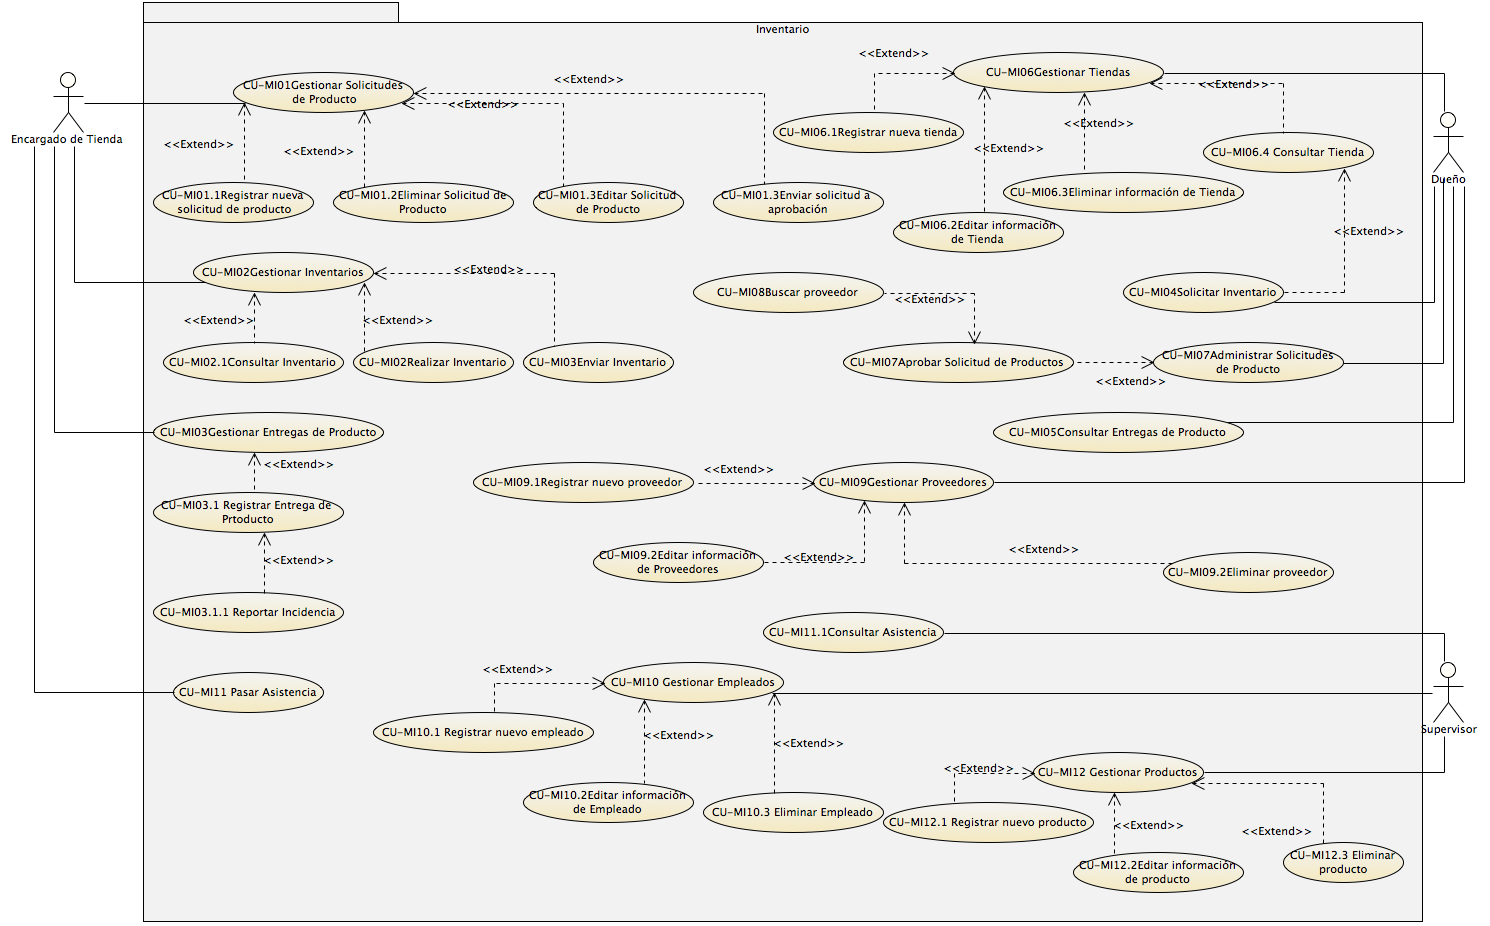
\includegraphics[width=\textwidth]{requerimientos/img/CU-MInventario}}
		\label{fig:Escenarios}
		\caption{Casos de Uso identificados y definidos para el módulo de Inventario}
	\end{center}
\end{figure}